\documentclass{beamer}
\usepackage{xcolor}
%\usepackage{fontspec}
%\setmainfont{Georgia}
%\usepackage[T1]{fontenc}
\usepackage{winfonts}
\usepackage[backend=bibtex]{biblatex}
\renewcommand{\sfdefault}{georgia}

\bibliography{report}

%%%%%%%%%%%%%%
% Soton colourscheme

%primary palette:           RED    GREEN  BLUE
\definecolor{sotonblu}{rgb}{.00392 .26275 .34902} % soton blue
\definecolor{sotongrn}{rgb}{.00000 .44706 .45882} % soton green
\definecolor{sotoncya}{rgb}{.03922 .58824 .66275} % soton cyan
\definecolor{sotongry}{rgb}{.19608 .23922 .26275} % soton grey
\definecolor{sotonbei}{rgb}{.59216 .61961 .27059} % soton beige
\definecolor{sotonmet}{rgb}{.73333 .73333 .73333} % soton metal

%some secondary colors:
\definecolor{sotonyel}{rgb}{.99999 .70196 .00000} % soton yellow
\definecolor{sotonora}{rgb}{.99608 .24314 .07843} % soton orange
\definecolor{sotonred}{rgb}{.94118 .05882 .17255} % soton red
\definecolor{sotonrus}{rgb}{.67059 .07059 .06275} % soton russet
\definecolor{sotonbrn}{rgb}{.54118 .25490 .16863} % soton brown
\definecolor{sotonpnk}{rgb}{.88627 .41176 .62353} % soton pink
\definecolor{sotonppl}{rgb}{.32549 .12157 .26667} % soton purple


\setbeamertemplate{background canvas}[vertical shading][top=sotonblu,bottom=sotoncya]
\setbeamercolor{background canvas}{bg=}
\setbeamercolor{button border}{bg=sotonblu, fg=sotonblu}
\setbeamercolor{button}{bg=sotonblu, fg=DarkRed}

\setbeamercolor{frametitle}{fg=sotonyel}
\setbeamercolor{alerted text}{fg=sotonyel}
\setbeamercolor{normal text}{fg=white}
\setbeamercolor{titlelike}{fg=sotonyel}
\setbeamercolor{author}{fg=white}
\setbeamercolor{date}{fg=white}
\setbeamercolor{item}{fg=white}

%%%%%%%%%%%%%%%%%%%%

\title{Identification of the Curie Temperature Distribution from
Temperature Dependent Magnetisation Data}
\author{Jonathon Waters\inst{1}, Hans Fangohr\inst{1}, Denis Kramer\inst{1} and Ondrej Hovorka\inst{1}}
\institute{
	\inst{1}
	Engineering and the Environment,\\
	University of Southampton,\\
	UK
}

\begin{document}
\frame{\titlepage 

\includegraphics[height=1cm]{Images/sponsor-wo}\hfill
\includegraphics[height=1cm]{Images/uos_grey_large}}

\setbeamertemplate{headline}{
	\vskip25pt % horizontal line
	\vskip-21pt\hspace{2pt}\hfill
\includegraphics[height=7mm]{Images/sponsor-wo}\hspace{3.5mm}
\includegraphics[height=7mm]{Images/uos_grey_large}\hspace{3.5mm} % logo on the right
}

\setbeamertemplate{footline}{
	\vskip-8pt % horizontal line
	\hspace{12cm} \insertframenumber/\inserttotalframenumber
	\vskip4pt
}

\begin{frame}
	\frametitle{Introduction}
	\begin{columns}
		\column{7cm}
		\begin{itemize}
			\item{In HAMR (heat assisted magnetic recording) there is no fixed $T_C$ (Curie Temperature). It varies based upon a number of factors and leads to a distribution $f(T_C)$.}
			\item{The recording performance is greatly decreased in systems with a wide $f(T_C)$.}
			\item{According to a 2014 publication, understanding the distribution $f(T_C)$ is a key step to realising HAMR.\footnotemark[1]}
		\end{itemize}
		\column{5cm}
		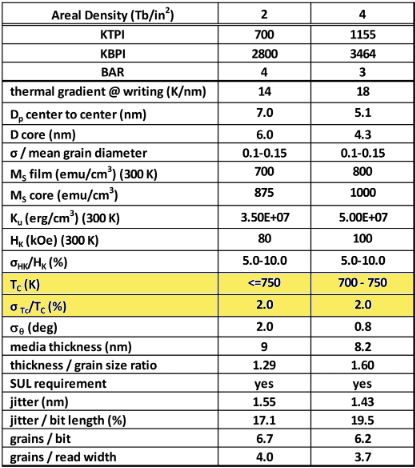
\includegraphics[width=5cm]{Images/Table}\footnotemark[1]
	\end{columns}
	\footnotetext[1]{\fullcite{weller2014hamr}}
\end{frame}

\begin{frame}
	\frametitle{Introduction}
	\begin{columns}
		\column{7cm}
		\begin{itemize}
			\item{HAMR material can be thought of as a collection of disconnected grains, each with different size $D$.\newline}
			\item{As the grain size approaches HAMR levels, $T_C$ becomes dependent upon $D$, resulting in a distribution in $T_C$.\newline}
			\item{We present a method to identify $f(T_C)$ from the magnetisation of the entire assembly.}
		\end{itemize}
		\column{5cm}
		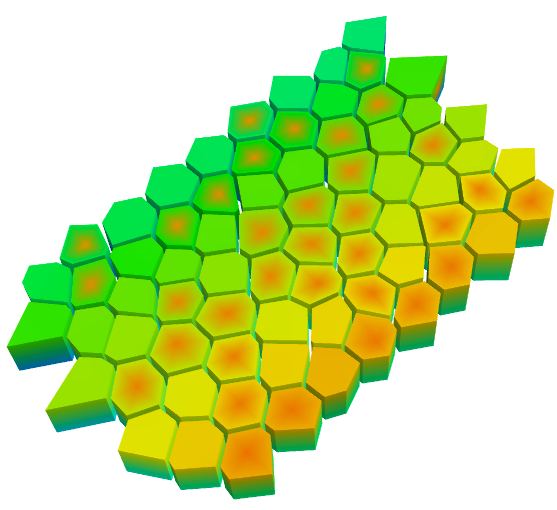
\includegraphics[width=5cm]{Images/grains}
	\end{columns}
\end{frame}

\begin{frame}
	\frametitle{Previous Methods}
\end{frame}

\begin{frame}
	\frametitle{Objectives}
	\begin{itemize}
		\item{Develop a method to identify the $T_C$ distribution which incorporates the finite size effects of the individual grains.\newline}
		\item{Test this method against a toy model in order to verify it's effectiveness.\newline}
		\item{Test the sensitivity of the model against various grain size distributions.\newline}
	\end{itemize}
\end{frame}

\begin{frame}
	\frametitle{Our Method}
	We assume that the magnetisation of an individual grain obeys the finite size scaling function:\footfullcite{hovorka2012curie}
	$$
	m(D,T) \propto D^{-\beta/\nu} \mu \left(D^{1/\nu}\frac{T-T_C^b}{T_C^b}\right)
	$$
	where $\beta$ and $\nu$ are \textit{universal exponents}, $\nu$ is the \textit{universal scaling function} and $T_C^b$ is the bulk Curie temperature.
	
	Taking the average of these magnetisations over all grain sizes leads to the form of the ensemble magnetisation for the 2D case:
	$$
	M(T) = M_0\int_0^\infty D^{2 - \beta/\nu} \mu \left(D^{1/\nu}\frac{T-T_C^b}{T_C^b}\right) f_D(D) dD
	$$
\end{frame}

\begin{frame}
	\frametitle{Our Method}
	Using the change of variables:
	$$
	t \equiv T_C^b - T_C(D) = T_C^b \left(\frac{D}{d_0}\right)^{-1/\nu}
	$$
	where $d_0$ is the \textit{length scale calibration factor}, close to the unit cell length, we can rewrite the ensemble magnetisation as:
	$$
	M(T) = M_0^*\int_0^{T_C^b} t^{-2\nu +\beta} \mu\left(d_0^{\frac{1}{\nu}}\frac{T-T_C^b}{t}\right) f_t(t) dt
	$$
	which can be fitted to magnetisation measurements for ensemble material in order to find $f_t(t)$.
\end{frame}

\begin{frame}
	\frametitle{Test Case: 2D Ising Model}
	\begin{columns}
	\column{7cm}
		The method we introduced was tested against the 2D Ising model in order to verify it's effectiveness:
		\begin{itemize}
		\item{Individual grain sizes were modelled using Metropolis Monte Carlo simulations.}
		\item{The universal constants and function were found by collapsing the curves for individual grain sizes onto the universal function.}
		\item{The universal exponents found were consistent with the analytical exponents of the 2D Ising model.}
		\end{itemize}
	\column{5cm}
		GRAIN PICTURE HERE
		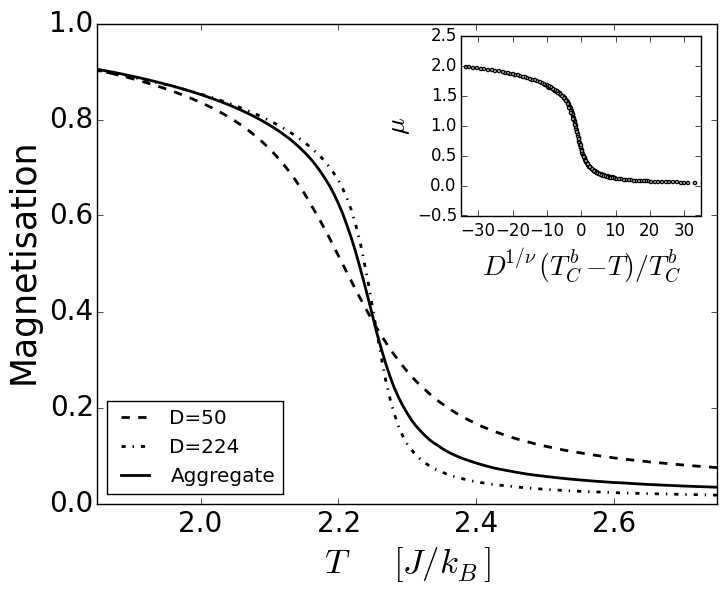
\includegraphics[width=5cm]{Images/Ds}
	\end{columns}
\end{frame}

\begin{frame}
	\frametitle{Test Case: 2D Ising Model}
	\begin{columns}
	\column{7cm}
		\begin{itemize}
		\item{A seperate Monte Carlo simulation was then run which modelled an assembly of grains with a lognormal grain size distribution ($\bar{D}=100$ and $\sigma_D=30$).}
		\item{The resultant distribution was then compared against that which was directly converted from the known distribution in $D$.}
		\item{After the success of this fit, other distributions in $D$ were attempted.}
		\end{itemize}
	\column{5cm}
		TC DISTRIBUTIONS
	\end{columns}
\end{frame}

\begin{frame}
	\frametitle{Test Case: 2D Ising Model}
	\begin{columns}
	\column{7cm}
		\begin{itemize}
		\item{It can be seen that the fit becomes poorer as the size distribution narrows.}
		\item{A constrained fit was attempted in order to correct this. If $\sigma_D/\bar{D}$ is known, then $\bar{t}$ can be fixed. $d_0$ can then be found by fitting $T_C(D)$, meaning that only $M_0^*$ and $\sigma_t$ need to be fitted.}
		\end{itemize}
		$$
		T_C(D) = T_C^b\left(1 - \left(\frac{D}{d_0}\right)^{-1/\nu}\right)
		$$
	\column{5cm}
		DISTRO SOLUTIONS
	\end{columns}
\end{frame}

\begin{frame}
	\frametitle{Conclusions}
\end{frame}

\begin{frame}
	\frametitle{Acknowledgements}
	In the completion of this work, we acknowledge financial support from the EPSRC Centre for Doctoral Training grant EP/L006766/1. \newline
	
	We also acknowledge the use of the IRIDIS High Performance Computing Facility, and associated support services at the University of
Southampton. \newline

	Contact: J.M.Waters@soton.ac.uk
\end{frame}
\end{document}